
\documentclass{scrreprt}
\usepackage{amsmath}
\usepackage{listings}
\usepackage{array}
\usepackage{tikz} 
\usepackage{underscore}
\usepackage[bookmarks=true]{hyperref}
\usepackage[utf8]{inputenc}
\usepackage[english]{babel}
\usepackage{enumitem}
\usepackage[a4paper, margin=1in]{geometry}
\usetikzlibrary{shapes, arrows.meta, positioning, backgrounds}

% Define styles for different node types
\tikzstyle{startstop} = [rectangle, rounded corners, minimum width=3cm, minimum height=1cm, text centered, draw=black, fill=red!30]
\tikzstyle{process} = [rectangle, minimum width=3.5cm, minimum height=1cm, text centered, draw=black, fill=blue!30]
\tikzstyle{arrow} = [thick,->,>=stealth]

% Define stickman style
\tikzset{
    stickman/.pic={
        % Head
        \draw[fill=gray] (0,0.6) circle (0.3cm);
        % Body
        \draw[line width=0.5mm] (0,0.3) -- (0,-0.6);
        % Arms
        \draw[line width=0.5mm] (-0.4,0.3) -- (0.4,0.3);
        % Legs
        \draw[line width=0.5mm] (0,-0.6) -- (-0.4,-1.2);
        \draw[line width=0.5mm] (0,-0.6) -- (0.4,-1.2);
    }
}

% Hyperref settings
\hypersetup{
    pdftitle={Software Requirement Specification},
    pdfauthor={Jean-Philippe Eisenbarth},
    pdfsubject={TeX and LaTeX},
    pdfkeywords={TeX, LaTeX, graphics, images},
    colorlinks=true,
    linkcolor=blue,
    citecolor=black,
    filecolor=black,
    urlcolor=purple,
    linktoc=page
}

% Set extra row height and padding
\setlength{\extrarowheight}{4pt}
\renewcommand{\arraystretch}{1.5}

\begin{document}

\begin{titlepage}
    \centering
    \includegraphics[width=0.5\textwidth]{logo.png} % Adjust width as necessary
    \vspace{1cm}

    \textbf{Department of Computer Science and Engineering}\\
    Premier University
    \vspace{1cm}

    \huge \textnormal{CSE 364: Data Communication}
    \vspace{1in} % Adjusts vertical space after the course title

    \Large \textnormal{Title: Complex Engineering Assignment}
    \vspace{0.5in} % Adjusts vertical space after the assignment title

    \large
    \textbf{Submitted by:}
    \vspace{0.5cm}

    \renewcommand{\arraystretch}{1.5} % Adjusts vertical spacing in the table
    \begin{tabular}{|p{0.4\textwidth}|p{0.6\textwidth}|} % Set column widths to 40% and 60%
        \hline
        \textbf{Name} & Mohammad Hafizur Rahman Sakib\\
        \hline
        \textbf{ID} & 0222210005101118 \\
        \hline
        \textbf{Section} & C \\
        \hline
        \textbf{Session} & Fall 2024 \\
        \hline
        \textbf{Semester} & 6th Semester \\
        \hline
        \textbf{Submission Date} & 20.03.2025 \\
        \hline
    \end{tabular}
    \vspace{1cm}

    \begin{minipage}[t]{0.48\textwidth}
        \textbf{Submitted to:}\\
        Estiak Ahamed Sazid\\
        Lecturer, Department of CSE\\
        Premier University\\
        Chittagong
    \end{minipage}%
    \hfill
    \begin{minipage}[t]{0.48\textwidth}
        \raggedleft
        \textbf{Remarks}\\
        \vspace{0.5cm} % Adjust vertical space for remarks
        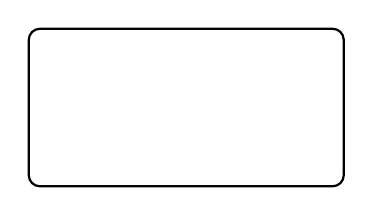
\begin{tikzpicture}
            \draw[thick, rounded corners] (0,0) rectangle (4,2);
        \end{tikzpicture}
    \end{minipage}

    \date{\today}
    \vfill
\end{titlepage}

\end{document}